%!TEX root = ./workbook-2011.tex

\section{Basic statistical functions in R}

\subsection{Dealing with Data Subsets in R}

Manipulating or analyzing subsets of data is one of the most common
tasks in R. The \lstinline!subset()! function comes in handy for such
operations. Consider the data set \lstinline!turtles.txt!:
%
\begin{R}
> turtles <- read.table('turtles.txt', header=T)
> turtles
   sex length width height
1    f     98    81     38
2    f    103    84     38
3    f    103    86     42
  # output truncated
> names(turtles)
[1] "sex"    "length" "width"  "height"
> # Now we'll apply the subset() function
> turt.sub <- subset(turtles, select = -sex)
> names(turt.sub)
[1] "length" "width"  "height"
> turt.sub
   length width height
1      98    81     38
2     103    84     38
3     103    86     42
  # output truncated
\end{R}
%
In the example above we create a subset of the original data set by
excluding the variable indicating the sex of each individual using the
argument \lstinline!select = -sex!. We can also explicit include only
certain variables, like this:
%
\begin{R}
> turt.sub2 <- subset(turtles, select=c(height,width))
> turt.sub2
   height width
1      38    81
2      38    84
3      42    86
  # output truncated    
\end{R}
%
\lstinline!subset()! allows you to do more than just select variables to
include. You can use the second positional argument to specify matching
criteria. For example:
%
\begin{R}
# gives only female turtles, all variables except sex
> female.turts <- subset(turtles, sex == "f", select = -sex)
> dim(female.turts)
[1] 24  3
# same for male turtles
> male.turts <- subset(turtles, sex == "m", select = -sex)
> dim(male.turts)
[1] 24  3
# gives only females with length > 125, all variables
> big.females <- subset(turtles, sex == "f" & length > 125)    
\end{R}

The \lstinline!subset! function is especially useful when combined with
the function \lstinline!sapply()! which allows you to apply a function
of interest to each variable. For example:
%
\begin{R}
> min(turtles)
Error in Summary.data.frame(..., na.rm = na.rm) : 
        only defined on a data frame with all numeric or complex variables
> min(turt.sub)  # unexpected result
[1] 35
> sapply(turt.sub, min) # here's what we were shooting for
length  width height 
    93     74     35
> sapply(female.turts, min) # for females
length  width height 
    98     81     38 
> sapply(male.turts, min) # for males
length  width height 
    93     74     35      
\end{R}
%
Notice how the \lstinline!min()! function chokes on the complete data
set because the function is not defined for factor variables. In the
second example \lstinline!min(turt.sub)! returns a valid result, but
also not exactly what we wanted. In this case it looked for the minimum
value across all the objects passed to it. In the third case we use the
\lstinline!sapply()! function and get the minimum on a
variable-by-variable basis. Please take a moment to look at the
documentation for the \lstinline!sapply()! function and cook up some
examples of your own.

\paragraph{Anderson's (Fisher's) iris data set}

Anderson's (or Fisher's) iris data set consists of four morphometric
measurements for specimens from three different iris species. Use the R
help to read about the iris data set (\lstinline!?iris!). We'll be using
this data set repeatedly in future weeks so familiarize yourself with
it.

\smallskip
\begin{assignment}
Calculate a summary table as well as correlation
and covariance matrices for each of the species in the iris data set.
Use \lstinline!help.search()! and \lstinline!apropos()! to lookup any
necessary function names.
\end{assignment}


\subsection{Exploring Univariate Distributions in R}

\subsubsection{Histograms}

One of the most common ways to examine a the distribution of
observations for a single variable is to use a histogram. The
\lstinline!hist()! function creates simple histograms in R.

\begin{R}
> hist(turtles$length) # create histogram with fxn defaults
> ?hist # check out the documentation on hist
\end{R}
Note that by default the \lstinline!hist()! function plots the
frequencies in each bin. If you want the probability densities instead
set the argument \lstinline!freq=FALSE!.
%
\begin{R}
> hist(turtles$length,freq=F) # y-axis gives probability density
\end{R}
Here's some other ways to fine tune a histogram in R.

\begin{R}
> hist(turtles$length, breaks=12) # use 12 bins
> mybreaks = seq(85,185,8)
> hist(turtles$length, breaks=mybreaks) # specify bin boundaries   
> hist(turtles$length, breaks=mybreaks, col='red') # fill the bins with red  
\end{R}

\subsubsection{Density Plots}

One of the problems with histograms is that they can be very sensitive
to the size of the bins and the break points used. This is due to the
discretization inherent in a histogram. A `density plot' or `density
trace' is a continuous estimate of a probability distribution from a set
of observations. Because it is continuous it doesn't suffer from the
same sensitivity to bin sizes and break points. One way to think about a
density plot is as the histogram you'd get if you averaged many
individual histograms each with slightly different breakpoints.
%
\begin{R}
> d <- density(turtles$length)
> plot(d)    
\end{R}
%
A density plot isn't entirely parameter free -- the parameter you should
be most aware of is the `smoothing bandwidth'.

\begin{R}
> d <- density(turtles$length) # let R pick the bandwidth
> plot(d,ylim=c(0,0.020)) # gives ourselves some extra headroom on y-axis
> d2 <- density(turtles$length, bw=5) # specify bandwidth
> lines(d2, col='red') # use lines to draw over previous plot
\end{R}
The bandwidth determines the standard deviation of the `kernel' that is
used to calculate the density plot. There are a number of different
types of kernels you can use; a Gaussian kernel is the R default and is
the most common choice. See the documentation for more info.

The \lstinline!lattice! package is an R library that makes it easier to
create graphics that show conditional distributions. Here's how to
create a simple density plot using the \lstinline!lattice! package.

\begin{R}
> library(lattice)
> densityplot(turtles$length) # densityplot defined in lattice
\end{R}
Notice how by default the \lstinline!lattice! package also drew points
representing the observations along the x-axis. These points have been
`jittered' meaning they've been randomly shifted by a small amount so
that overlapping points don't completely hide each other. We could have
produced a similar plot, without the lattice package, as so:

\begin{R}
> d <- density(turtles$length)
> plot(d)
> nobs <- length(turtles$length)
> points(jitter(turtles$length), rep(0,nobs)) 
\end{R}
Notice that in our version we only jittered the points along the x-axis.
You can also combine a histogram and density trace, like so:

\begin{R}
> hist(turtles$length, 10, xlab='Carapace Length (mm)',freq=F)
> d <- density(turtles$length)
> lines(d, col='red', lwd=2) # red lines, with pixel width 2    
\end{R}
Notice the use of the \lstinline!freq=F! argument to scale the histogram
bars in terms of probability density.

Finally, let's some of the features of \lstinline!lattice! to produce
density plots for the `length' variable of the turtle data set,
conditional on sex of the specimen.

\begin{R}
> densityplot(~length | sex, data = turtles)    
\end{R}
There are a number of new concepts here. The first is that we used what
is called a `formula' to specify what to plot. In this case the formula
can be read as `length conditional on sex'. We'll be using formulas in
several other contexts and we discuss them at greater length below. The
\lstinline!data! argument allows us to specify a data frame or list so
that we don't always have to write arguments like
\lstinline!turtles$length! or \lstinline!turtles$sex! which can get a
bit tedious.

\subsubsection{Box Plots}

Another common tool for depicting a univariate distribution is a `box
plot' (sometimes called a box-and-whisker plot). A standard box plot
depicts five useful features of a set of observations: the median
(center most line), the upper and lower quartiles (top and bottom of the
box), and the minimum and maximum observations (ends of the whiskers).

\begin{figure}[htbp]
\centering
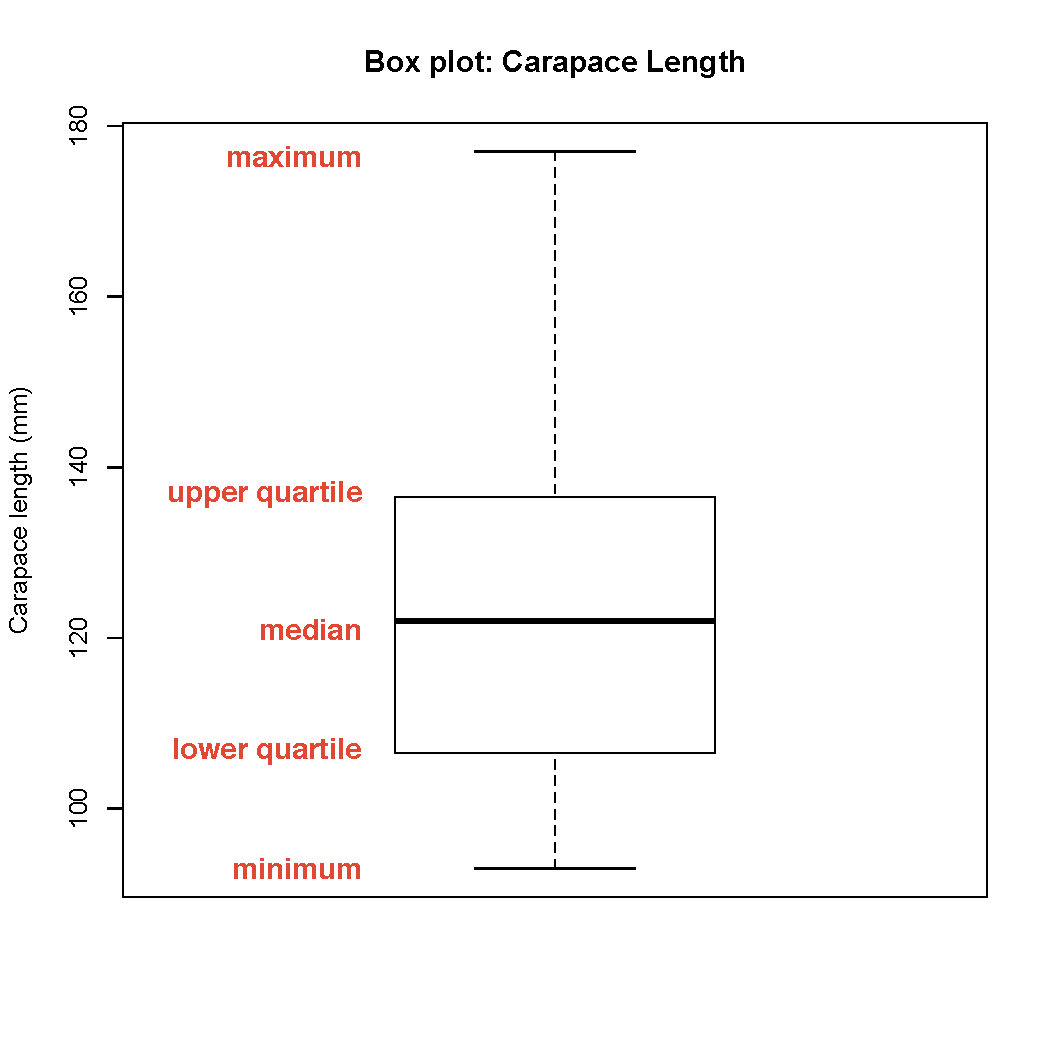
\includegraphics[width=0.5\columnwidth]{./figures/hands-on2/boxplot-labeled.pdf}
\caption{A box plot represents a five number summary of a set of
observations.}
\end{figure}

There are many variants on box plots, particularly with respect to the
`whiskers'. It's always a good idea to be explicit about what a box plot
you've created depicts.

Here's how to create box plots using the standard R functions as well as
the lattice package:

\begin{R}
> boxplot(turtles$length)
> boxplot(turtles$length, col='darkred', horizontal=T) # horizontal version 
> title(main = 'Box plot: Carapace Length', ylab = 'Carapace length (mm)')
> bwplot(~length,data=turtles) # using the bwplot function from lattice
\end{R}
Note how we used the \lstinline!title()! function to change the axis
labels and add a plot title.

\paragraph{Historical note}

-- The box plot is one of many inventions of the statistician John W.
Tukey. Tukey made many contributions to the field of statistics and
computer science, particularly in the areas of graphical representations
of data and exploratory data analysis.

\subsubsection{Bean Plots}

My personal favorite way to depict univariate distributions is called a
`beanplot'. Beanplots combine features of density plots and boxplots and
provide information rich graphical summaries of single variables. The
standard features in a beanplot include the individual observations
(depicted as lines), the density trace estimated from the observations,
the mean of the observations, and in the case of multiple beanplots an
overall mean.

\begin{figure}[htbp]
\centering
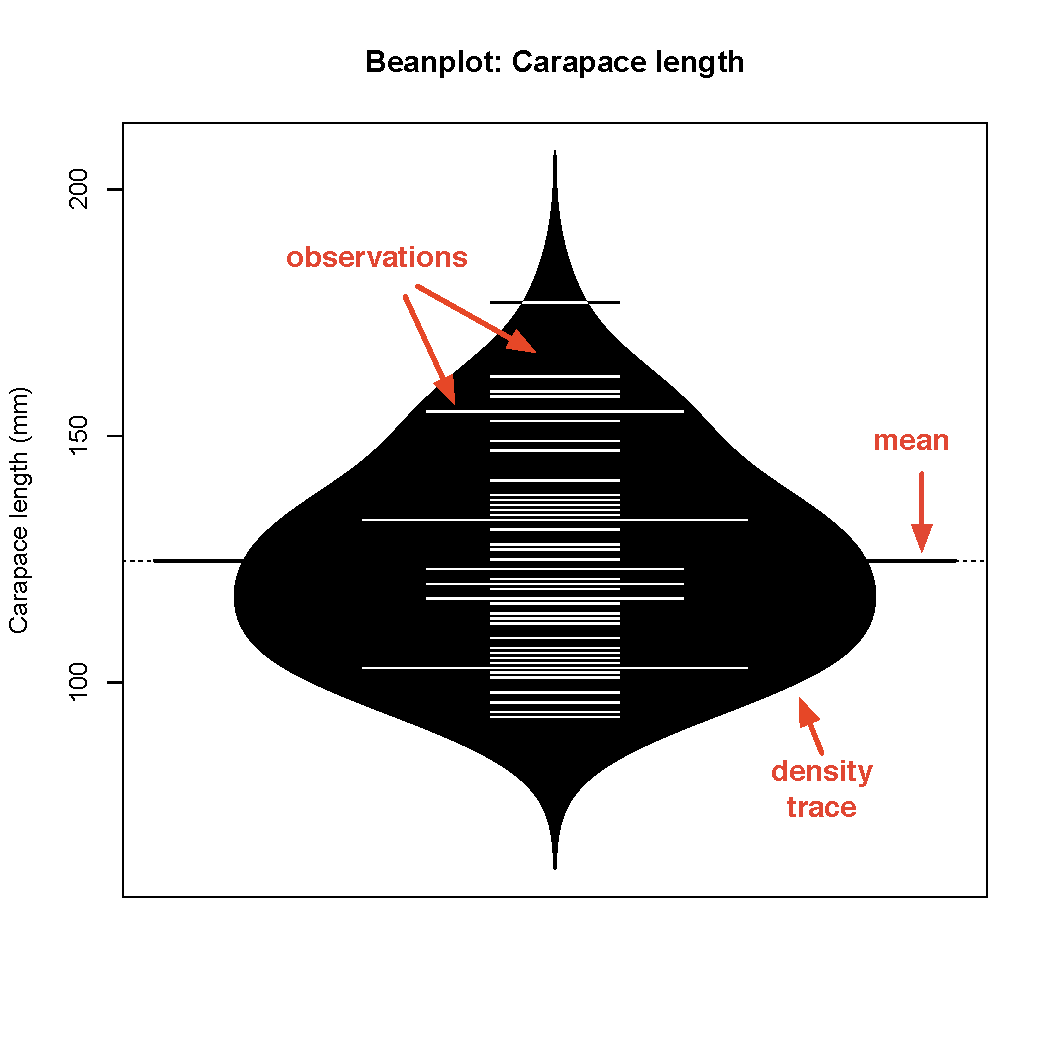
\includegraphics[width=0.5\columnwidth]{./figures/hands-on2/beanplot-labeled.pdf}
\caption{Beanplots combine features of density and box plots.}
\end{figure}

The \lstinline!beanplot! package is not installed by default. To
download it and install it use the R package installer under the
\lstinline!Packages & Data! menu (standard R GUI) or in
\lstinline!Tools > Install Packages...! in RStudio (see also the
\lstinline!Packages! tab in the lower-right window in RStudio). If this
is the first time you use the package installer you'll have to choose a
CRAN repository from which to download package info (I recommend you
pick one in the US). Once you've done so you can search for `beanplot'
from the Package Installer window. You should also check the 'install
dependencies' check box.

Once the beanplot package has been installed check out the examples to
see some of the capabilities:

\begin{R}
> library(beanplot) 
> example(beanplot)    
\end{R}
If you ran the examples in RStudio, use the \lstinline!Clear All! option
in the \lstinline!Plots! tab after running the examples in order to
reset parameters that the examples changed.

Note the use of the \lstinline!library()! function to make the functions
in the \lstinline!beanplot! library available for use. Here's some
examples of using the \lstinline!beanplot! function with the turtle data
set:

\begin{R}
> beanplot(turtles$length) # note the message about log='y'
> beanplot(turtles$length, log='') # DON'T do the automatic log transform
> beanplot(turtles$length, log='', col=c('white','blue','blue','red'))
\end{R}
In the final version we specified colors for the parts of the beanplot.
See the explanation of the \lstinline!col! argument int he beanplot
function for details.

We can also compare the carapace length variable for male and female
turtles.

\begin{R}
> beanplot(length ~ sex, data = turtles, col=list(c('red'),c('black')),
names = c('females','males'),xlab='Sex', ylab='Caparace length (mm)')
\end{R}
Note the use of the formula notation to compare the carapace length
variable for males and females. There is also a asymmetrical version of
the beanplot which can be used to more directly compare distributions
between two groups. We explore this below. Note too the use of the list
argument to \lstinline!col!, and the use of vectors within the list to
specify the colors for female and male beanplots.

We can also create a beanplot with multiple variables in the same plot
if the variables are measured on the same scale.

\begin{R}
> beanplot(turtles$length, turtles$width, turtles$height, log='',
names=c('length','width','height'), ylab='carapace dimensions (mm)') 
\end{R}


\subsection{Simple t-tests in R}

Student's t-tests can be carried out in R using the function
\lstinline!t.test()!. The \lstinline!t.test()! function can perform one
and two-sample t-tests (i.e.~comparing a sample of interest against a
hypothesized mean, or comparing the means of two samples). The
\lstinline!t.test()! function also supports a `formula' interface for
two-sample t-tests similar to the \lstinline!lm(!) function.

\begin{R}
> t.test(width ~ sex, data=turtles)

        Welch Two Sample t-test

data:  width by sex 
t = 4.7015, df = 35.355, p-value = 3.862e-05
alternative hypothesis: true difference in means is not equal to 0 
95 percent confidence interval:
  8.122699 20.460634 
sample estimates:
mean in group f mean in group m 
      102.58333        88.29167 
\end{R}
The asymmetric version of the boxplot is very useful for comparing
distributions of the same variable between two groups. To generate such
plots use the argument \lstinline!side='both'! as an argument to
\lstinline!beanplot!.

\begin{R}
> beanplot(width ~ sex, data = turtles, side='both', col=list(c('red'),c('black')))  
\end{R}
As you can see this splits the beanplot in half for each group and puts
them back to back to facilitate comparison. The difference in the mean
of the two groups is visually obvious from the beanplot.

\begin{assignment}
\begin{enumerate}[a)]
\item
  Prepare beanplots showing samples grouped by \lstinline!Species! for
  each of the quantitative variables in the iris data set. Label the x-
  and y-axes of your boxplots and give each plot a title. \textbf{Tip}: since there are three species, you can't use the \lstinline!side='both'! argument, and you'll need to extend the \lstinline!col=list! argument to add a third color.

\item Carry out two-sample t-tests contrasting \lstinline!versicolor! and
  \lstinline!virginica! for each of the four morphometric variables in
  the iris data set. \textbf{Tip}: use the \lstinline!subset()! function to create a subset of the iris data containing just these two species.

\item Write a brief paragraph interpreting the results of the t-tests you
  conducted.
\end{enumerate}
\end{assignment}

\subsection{Exploring Bivariate Distributions in R}

\subsubsection{Scatterplots}

When dealing with pairs of continuous variables a scatter plot is the
obvious choice. The standard \lstinline!plot! function can be used:

\begin{R}
> plot(turtles$length, turtles$width)
> plot(turtles$length ~ turtles$width)    
\end{R}
Did you notice what is different between the two versions above? You can
also use the \lstinline!data! argument with plot, like so:

\begin{R}
> plot(length ~ width, data=turtles)
\end{R}
The \lstinline!xyplot()! function from the \lstinline!lattice! package
does pretty much the same thing:
%
\begin{R}
> xyplot(length ~ width, data = turtles)
\end{R}


\subsubsection{Regression in R}

R has very flexible built in functions for fitting linear models.
Bivariate regression is the simplest case of a linear model.

\begin{R}
> turtles <- read.table('turtles.txt',header=T)
> names(turtles)
[1] "sex"    "length" "width"  "height"
> regr <- lm(turtles$width ~ turtles$length)
> class(regr)
[1] "lm"
> names(regr)
 [1] "coefficients"  "residuals"     "effects"       "rank"          "fitted.values"
 [6] "assign"        "qr"            "df.residual"   "xlevels"       "call"         
[11] "terms"         "model"   
> summary(regr)

Call:
lm(formula = turtles$width ~ turtles$length)

Residuals:
     Min       1Q   Median       3Q      Max 
-5.57976 -1.66578 -0.04471  1.73752  5.97104 

Coefficients:
               Estimate Std. Error t value Pr(>|t|)    
(Intercept)     19.9434     2.3877   8.353 8.99e-11 ***
turtles$length   0.6055     0.0189  32.033  < 2e-16 ***
---
Signif. codes:  0 '***' 0.001 '**' 0.01 '*' 0.05 '.' 0.1 ' ' 1 

Residual standard error: 2.654 on 46 degrees of freedom
Multiple R-Squared: 0.9571,     Adjusted R-squared: 0.9562 
F-statistic:  1026 on 1 and 46 DF,  p-value: < 2.2e-16 

> plot(turtles$width ~ turtles$length)  # scatter plot with turtles$length on x axis
> abline(regr)  # plot the regression line
\end{R}
Note the use of the function \lstinline!abline()! to plot the regression
line. Calling \lstinline!plot()! with an object of class \lstinline!lm!
shows a series of diagnostic plots. Try this.

\begin{assignment}
Write your own regression function (i.e.~your
code shouldn't refer to the built in regression functions) for mean
centered vectors in R. The function will take as it's input two vectors,
$\vec{x}$ and $\vec{y}$. The function should return:

\begin{enumerate}[1.]
\item
  a list containing the mean-centered versions of these vectors
\item
  the regression coefficient $b$ in the mean centered regression
  equation $\vec{\widehat{y}} = b\vec{x}$
\item
  the coefficient of determination, $R^2$
\end{enumerate}
Demonstrate your regression function by using it to carry out
regressions of Sepal.Length on Sepal.Width separately for the `setosa'
and `virginica' specimens from the iris data set (again,
\lstinline!subset()! is your friend). Include plots in which you use the
\lstinline!plot()! and \lstinline!abline()! functions to illustrate your
calculated regression line.

\end{assignment}
